\documentclass{beamer}
\usepackage{hyperref}
\usepackage[T1]{fontenc}
% \usepackage{ctex}
\usepackage[english]{babel}
\usepackage{algorithm2e}
\usepackage{algorithmic}

\UseRawInputEncoding

% Cannot enable in Xelatex
\usepackage{pgfpages}
\usepackage{subcaption}
\usepackage{comment}
% \setbeameroption{hide notes} % Only slides
% \setbeameroption{show only notes} % Only notes
% \setbeameroption{show notes on second screen}

% other packages
\usepackage{latexsym,amsmath,xcolor,multicol,booktabs,calligra}
\usepackage{graphicx,listings,stackengine}
\usepackage{animate}

\definecolor{best}{rgb}{.8, .96, .94}
\usepackage{xcolor, colortbl}

% *************************** Additional package *****************************
\usepackage{multicol}
% \usepackage{subfigure}
\usepackage{comment}
\usepackage{verbatim}
\usepackage{multirow}

%% Enable only in Xelatex
% \usepackage{pstricks}

% Set hyperlink colors
\begin{comment}
\hypersetup{
    colorlinks=true,
    linkcolor=darkblue,  % Color para enlaces internos
    filecolor=darkblue,  % Color para enlaces a archivos
    urlcolor=darkblue    % Color para URLs
}
\end{comment}

\author[CIARC-2025]{CIARC-2025}

\title{Applications of Graph Neural Networks}
% \subtitle{Presentation}
\institute [LAAD] 
{
\vspace*{-0.1cm}
% 
\includegraphics[width=1.6cm]{pic/pucp.png}
\hspace*{0.25cm}~%
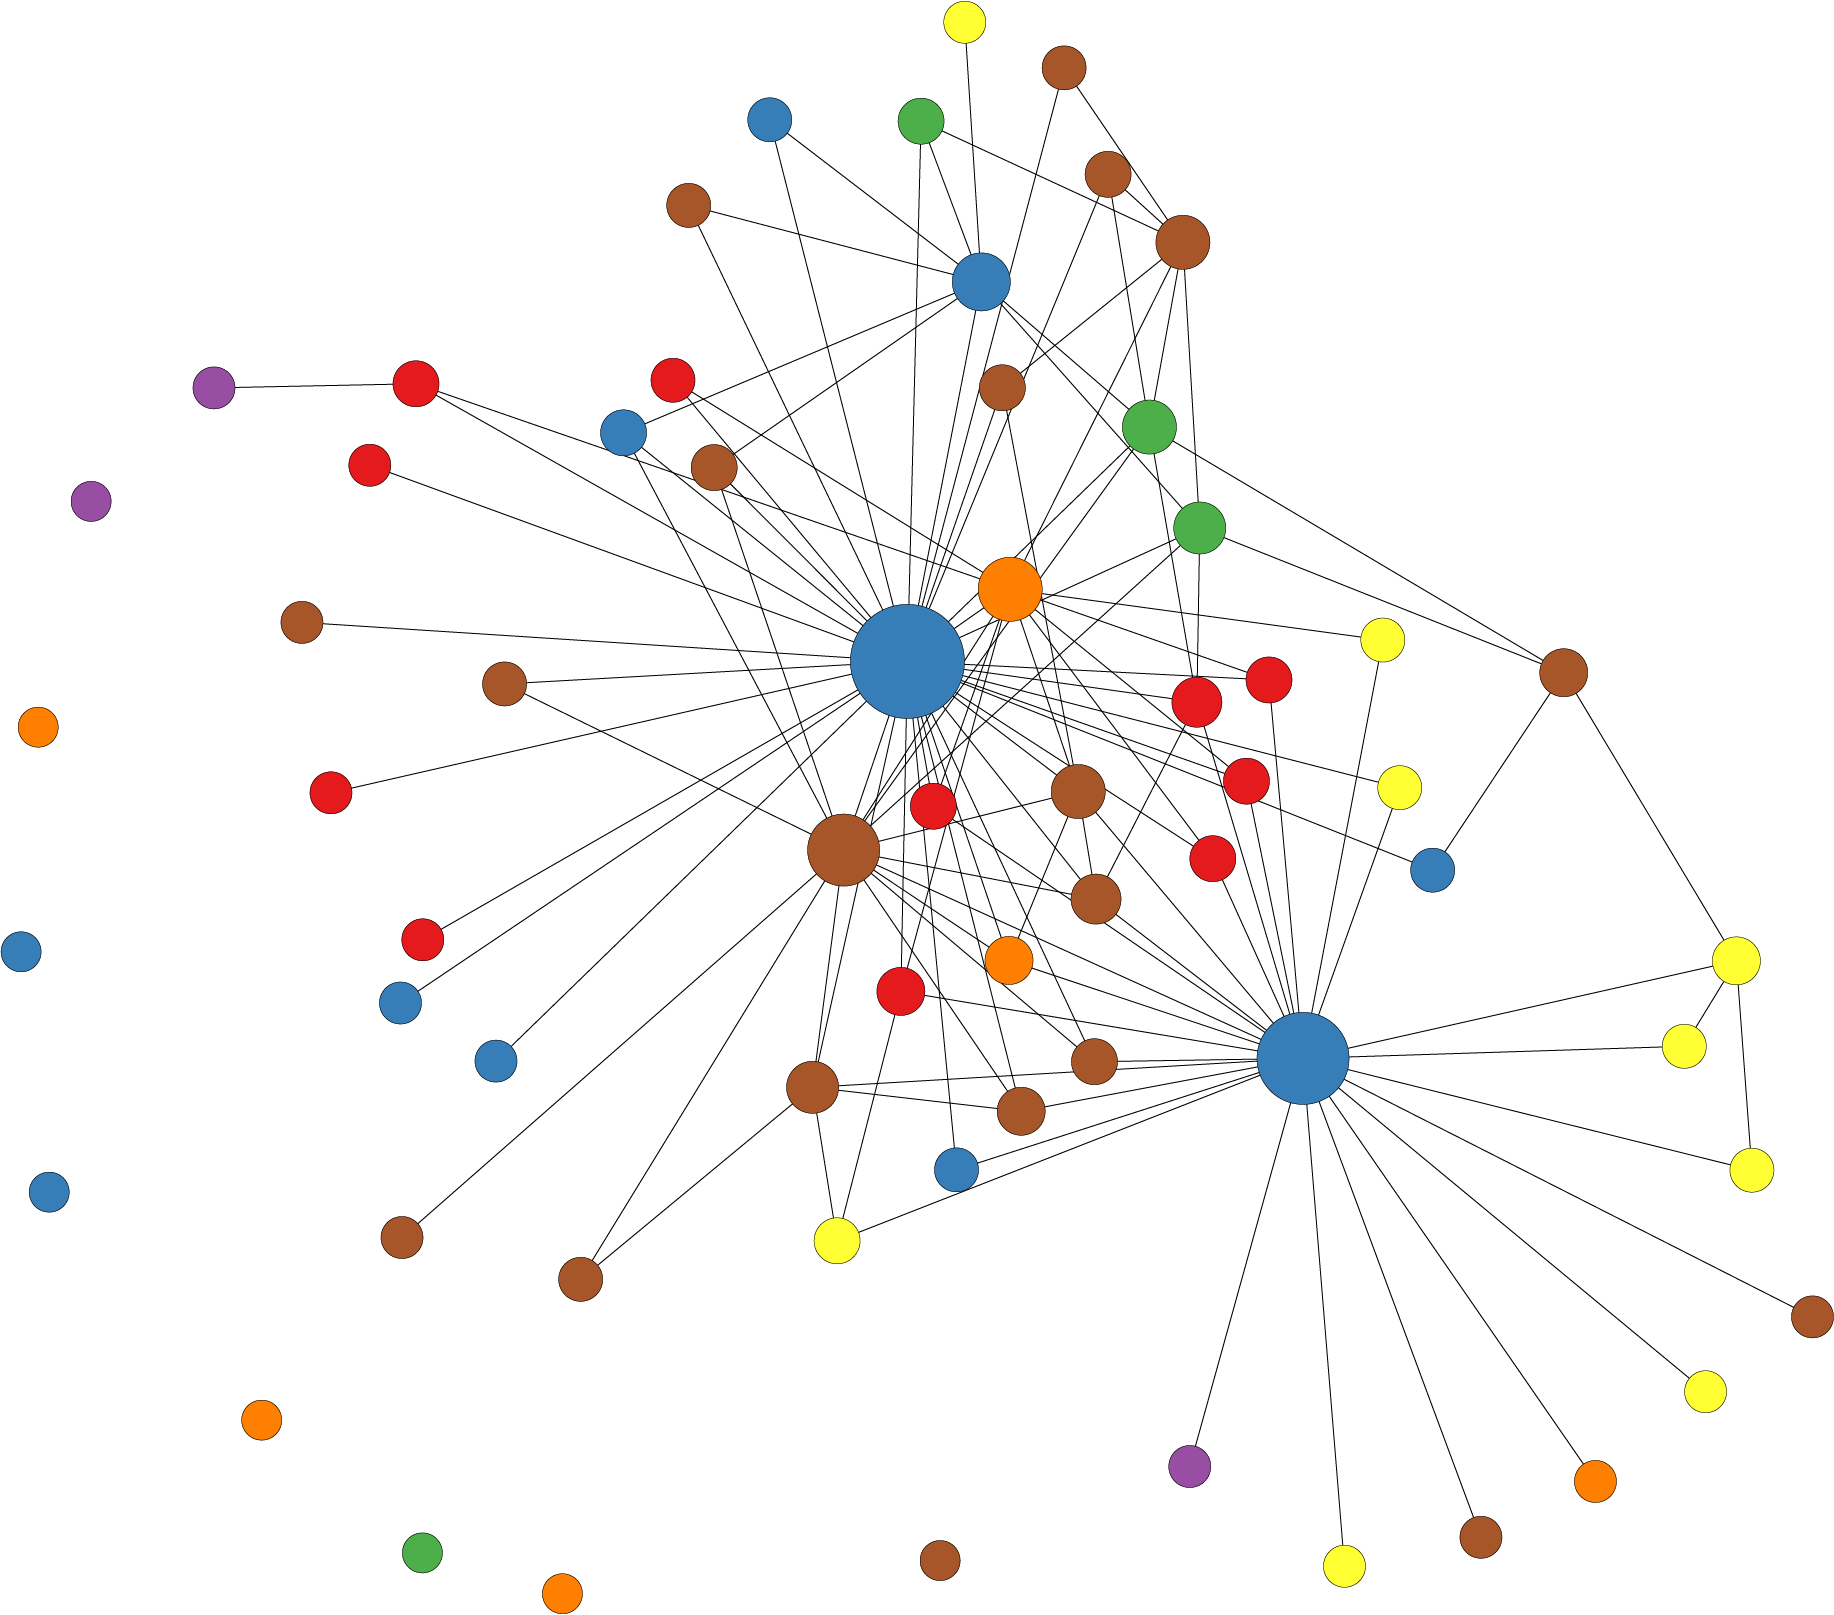
\includegraphics[width=2.0cm]{pic/logo_graph.png}
\hspace*{0.25cm}~%
% 
\includegraphics[width=1.4cm]{pic/unmsm.png}
\vspace*{0.35cm}\\

% Inteligencia Artificial PUCP (IA-PUCP)
}

\date{\scriptsize January 14, 2025}
\usepackage{YTU}

% defs
\def\cmd#1{\texttt{\color{red}\footnotesize $\backslash$#1}}
\def\env#1{\texttt{\color{blue}\footnotesize #1}}
\definecolor{deepblue}{rgb}{0,0,0.5}
\definecolor{deepred}{rgb}{0.6,0,0}
\definecolor{deepgreen}{rgb}{0,0.5,0}
\definecolor{halfgray}{gray}{0.55}

\lstset{
    basicstyle=\ttfamily\small,
    keywordstyle=\bfseries\color{deepblue},
    emphstyle=\ttfamily\color{deepred},    % Custom highlighting style
    stringstyle=\color{deepgreen},
    numbers=left,
    numberstyle=\small\color{halfgray},
    rulesepcolor=\color{red!20!green!20!blue!20},
    frame=shadowbox,
}

\begin{document}

\begin{frame}
    \titlepage
    \begin{figure}[ht!]
        \begin{center}
            % 
\includegraphics[width=0.2\linewidth]{pic/YTU_logo.jpg}
       \end{center}
    \end{figure}
    
    \begin{note}
        {Go...}
    \end{note}
\end{frame}

\begin{frame}
    \tableofcontents[sectionstyle=show,subsectionstyle=show/shaded/hide,subsubsectionstyle=show/shaded/hide]
    % \tableofcontents[sectionstyle=show,subsectionstyle=hide,subsubsectionstyle=hide]
\end{frame}

\section{Introduction}
    \begin{frame}{Graphs}
        Graph is a data structure and is defined by $G = (V, E)$, where $V$ is the set of nodes and $E$ is the set of edges.
        
        \begin{figure}[ht!]
            \centering
            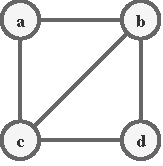
\includegraphics[width=0.25\linewidth]{pic/graph_example.pdf}
            \caption{\scriptsize Graph example.}
        \end{figure}
    \end{frame}
    
    \begin{frame}{Graph representations}
        \begin{figure}
            \centering
            \begin{subfigure}{0.241\textwidth}
                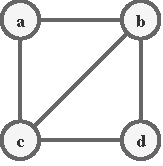
\includegraphics[width=\textwidth]{pic/graph_example.pdf}
                \caption{\tiny Input graph.}
                \label{fig:first}
            \end{subfigure}
            \hfill
            \begin{subfigure}{0.241\textwidth}
                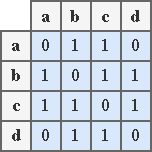
\includegraphics[width=\textwidth]{pic/graph_adjacency_matrix.pdf}
                \caption{\tiny Adjacency matrix.}
                \label{fig:second}
            \end{subfigure}
            \hfill
            \begin{subfigure}{0.241\textwidth}
                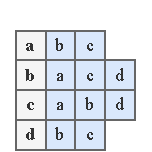
\includegraphics[width=\textwidth]{pic/graph_adjacency_list.pdf}
                \caption{\tiny Adjacency list.}
                \label{fig:third}
            \end{subfigure}
                    \hfill
            \begin{subfigure}{0.241\textwidth}
                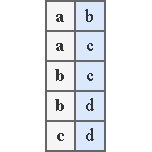
\includegraphics[width=\textwidth]{pic/graph_list_edge.pdf}
                \caption{\tiny Edge list.}
                \label{fig:third}
            \end{subfigure}
            \caption{\scriptsize Graph representations.}
            \label{fig:graph_representation}
        \end{figure}                     
    \end{frame}
    
    \begin{frame}{Other definitions/concepts}
        \begin{columns}
            \begin{column}{0.5\textwidth}
                \begin{itemize}
                    \item Homogeneous graph
                    \item Heterogeneous graph
                    \item Directed graph
                    \item Undirected graph
                    \item Weighted graph
                    \item Bipartite graph
                    \item Complete graph
                    \item Degree
                    \item Density
                    \item Diameter
                \end{itemize}
            \end{column}
            \begin{column}{0.5\textwidth}
                \begin{figure}[ht!]
                    \centering
                    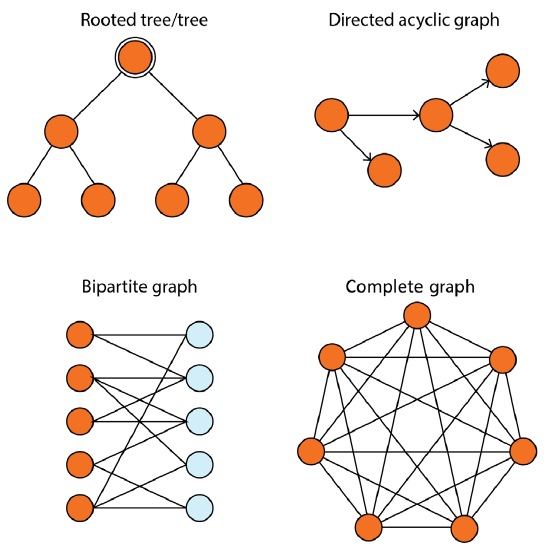
\includegraphics[width=1.0\linewidth]{pic/common_type_graph.png}
                    \caption{\scriptsize Common type of graphs. Adapted from \cite{labonne2023hands}.}
                    % \caption*{Adapted from \cite{labonne2023hands}.}
                \end{figure}
            \end{column}
        \end{columns}
        
        \note {Write your notes.\\}
        \begin{note}
            {Write your notes here}
        \end{note}
    \end{frame}

    \begin{frame}{Graphs are everywhere!}
        \begin{figure}[ht!]
            \centering
            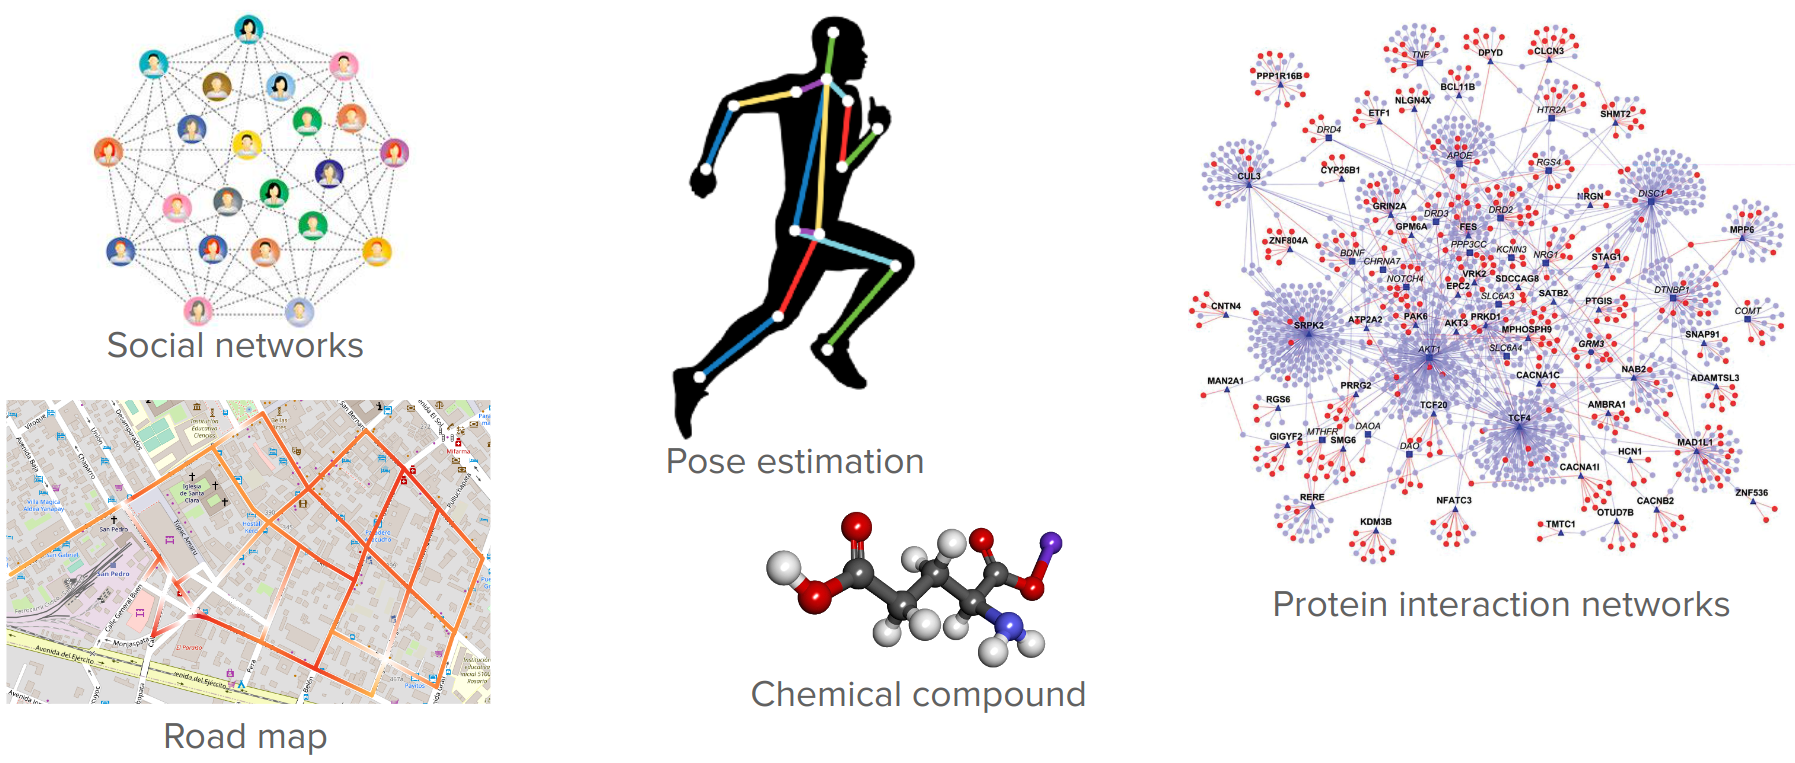
\includegraphics[width=1.0\linewidth]{pic/graphs_everywhere.png}
            \caption{\scriptsize Graphs are everywhere.}
        \end{figure}               
    \end{frame}

    \begin{frame}{Graph embedding}
        It is a function $f: A \rightarrow Z$ that maps each node of the graph $G = (V, E)$ into a $d$-dimensional vector. Where, $Z = \{z_1, z_2, ..., z_N\}$, $z_i \in \mathbb{R}^{d}$ with $d \ll N$. % Usually, $z_i$ and $Z$ are called node embedding and embedding matrix, respectively.

        \begin{figure}[ht!]
            \centering
            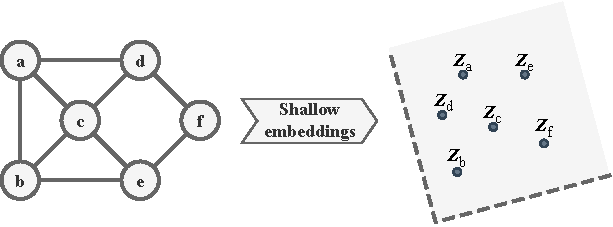
\includegraphics[width=0.7\linewidth]{pic/shallow_embeddings.pdf}
            \caption{\scriptsize Shallow embeddings scheme.}
        \end{figure}               
    \end{frame}

    \begin{frame}{More about embeddings}
        \begin{figure}[ht!]
            \centering
            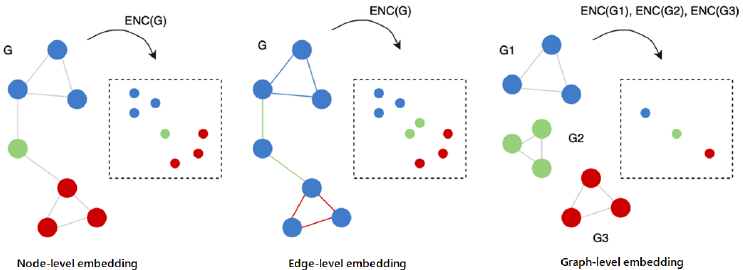
\includegraphics[width=1.0\linewidth]{pic/more_embeddings.png}
            \caption{\scriptsize Visual representation of the three different levels of granularity in graphs. Adapted from \cite{stamile2021graph}.}
        \end{figure}
                      
    \end{frame}

    \begin{frame}{Tasks}
        \begin{figure}[ht!]
            \centering
            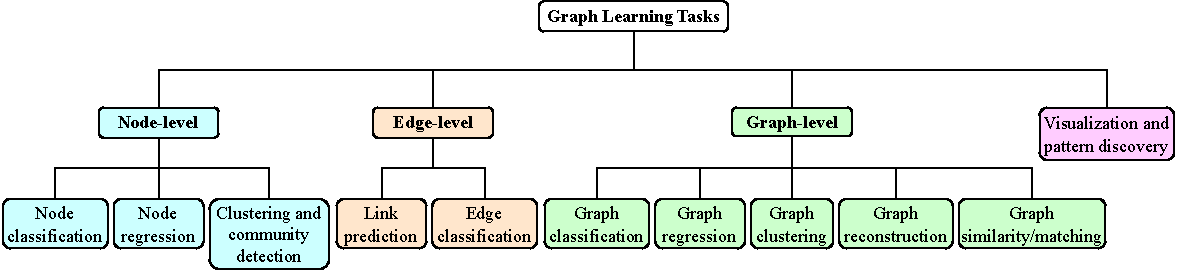
\includegraphics[width=1.0\linewidth]{pic/graph_learning_tasks.pdf}
            \caption{\scriptsize Overview of graph learning tasks.}
        \end{figure}               
    \end{frame}

    \begin{frame}{Tasks}
        \begin{figure}[ht!]
            \centering
            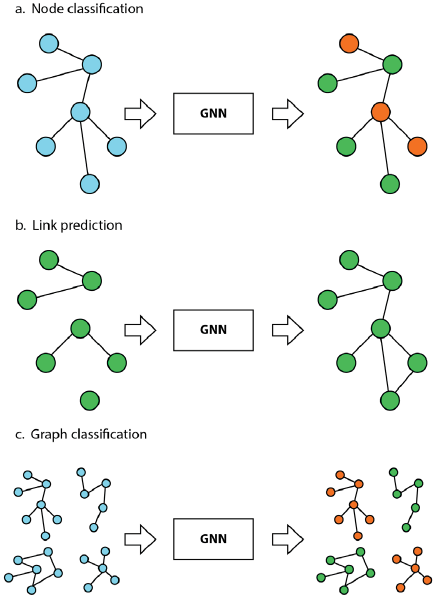
\includegraphics[width=0.43\linewidth]{pic/graph_learning_tasks_example.png}
            \caption{\scriptsize Examples of graph learning tasks. Adapted from \cite{labonne2023hands}.}
        \end{figure}               
    \end{frame}

    \begin{frame}{Applications}
        \begin{multicols}{2}
            \begin{itemize}
                \item Computer vision
                \item Natural language processing
                \item Recommender systems
                \item Program analysis
                \item Knowledge graphs
                \item Bioinformatics
                \item Chemistry
                \item Biology
                \item Physic
                \item Anomaly detection
                \item Urban intelligence
                \item Financial transaction
                \item ...
            \end{itemize}
        \end{multicols}          
    \end{frame}

    \begin{frame}{Taxonomy of graph machine learning methods.}
        \begin{figure}[ht!]
            \centering
            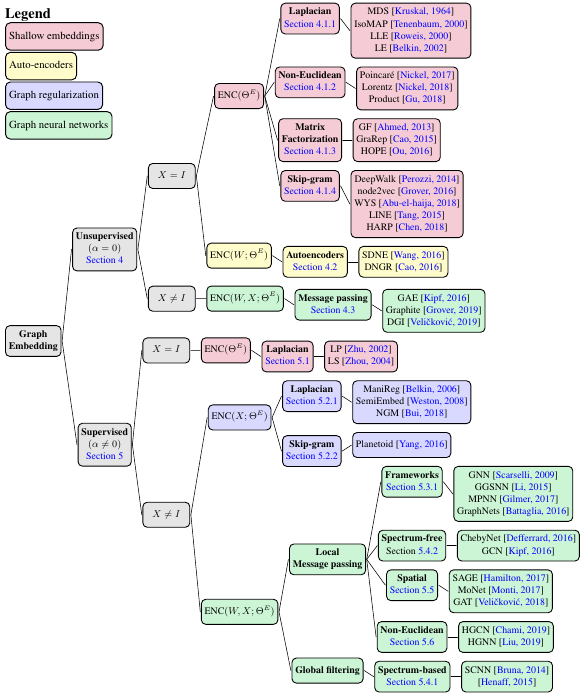
\includegraphics[width=0.512\linewidth]{pic/taxonomy_graph_machine_learning.png}
            \caption{\scriptsize Taxonomy of graph machine learning. Adapted from \cite{chami2022machine}.}
        \end{figure}               
    \end{frame}

\section{Traditional Method}
    \begin{frame}{Word2vec \cite{mikolov2013efficient}}
        \begin{figure}
            \centering
            \begin{subfigure}{0.4\textwidth}
                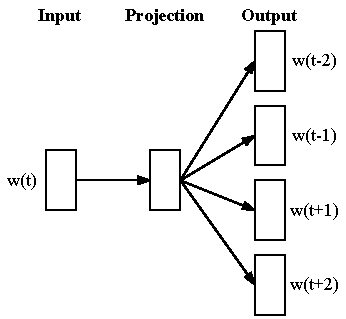
\includegraphics[width=\textwidth]{pic/skip_gram.pdf}
                \caption{\tiny Skip-gram.}
                \label{fig:first}
            \end{subfigure}
            \hfill
            \begin{subfigure}{0.4\textwidth}
                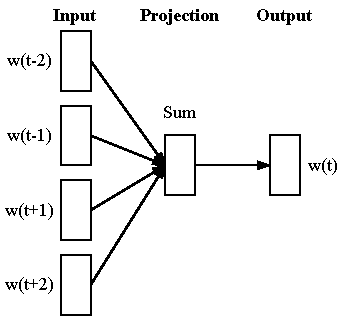
\includegraphics[width=\textwidth]{pic/cbow.pdf}
                \caption{\tiny CBOW.}
                \label{fig:third}
            \end{subfigure}
            \caption{\scriptsize Word embedding architectures. Adapted from \cite{mikolov2013efficient}.}
            \label{fig:word2vec_arquitecture}
        \end{figure} 
    \end{frame}

    \begin{frame}{Word2vec}   
        \begin{figure}[ht!]
            \centering
            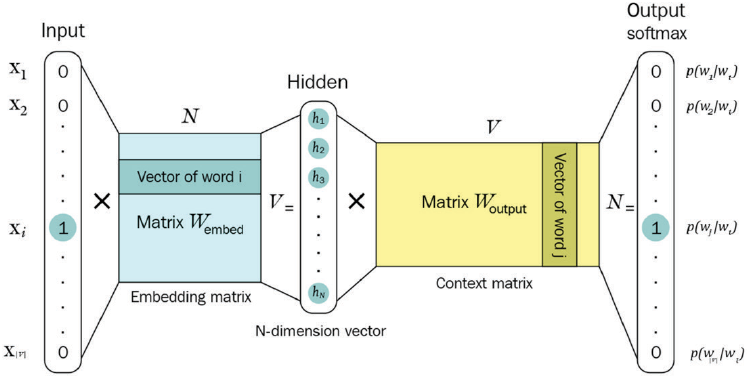
\includegraphics[width=0.9\linewidth]{pic/word2vec.png}
            \caption{\scriptsize Word2vec architecture. Adapted from \cite{labonne2023hands}.}
        \end{figure}   
    \end{frame}

    \begin{frame}{Word2vec in action}   
        \begin{figure}[ht!]
            \centering
            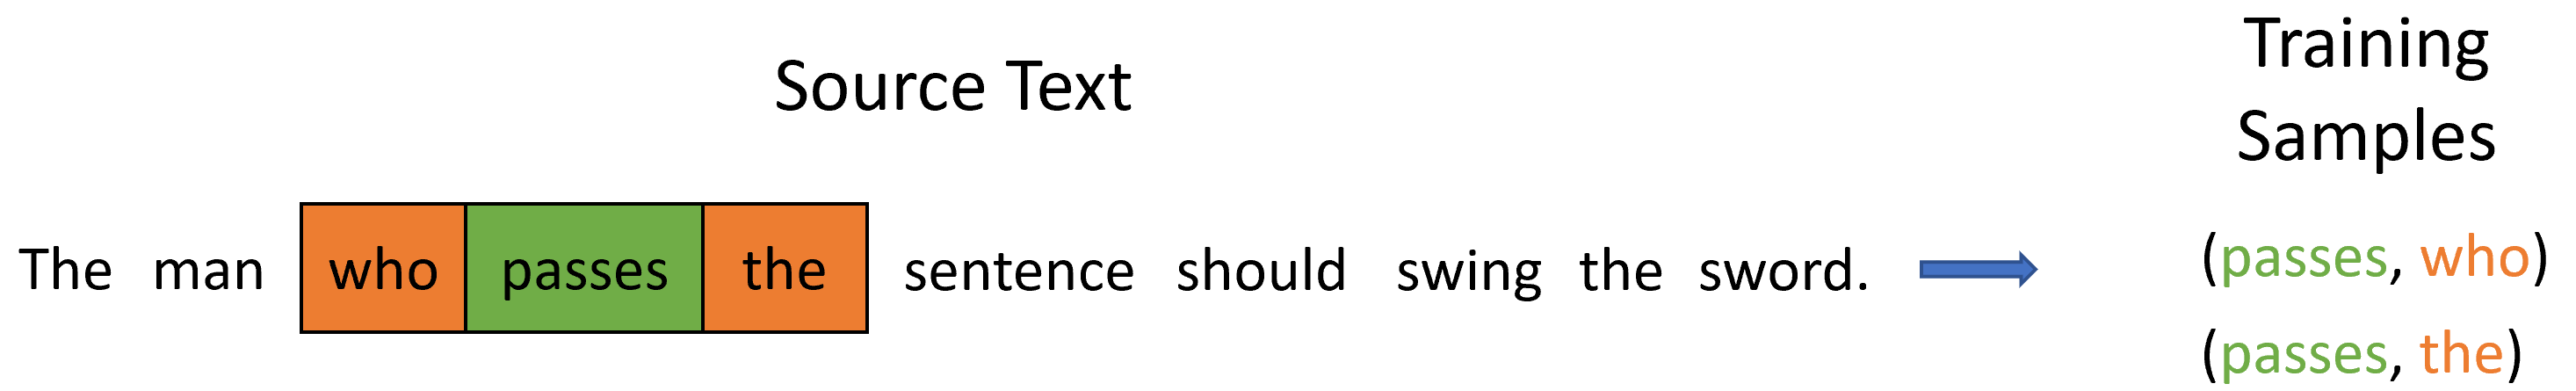
\includegraphics[width=0.65\linewidth]{pic/quote_ned_stark.png}
            \caption{\scriptsize Train window.}
        \end{figure}

        \begin{figure}[ht!]
            \centering
            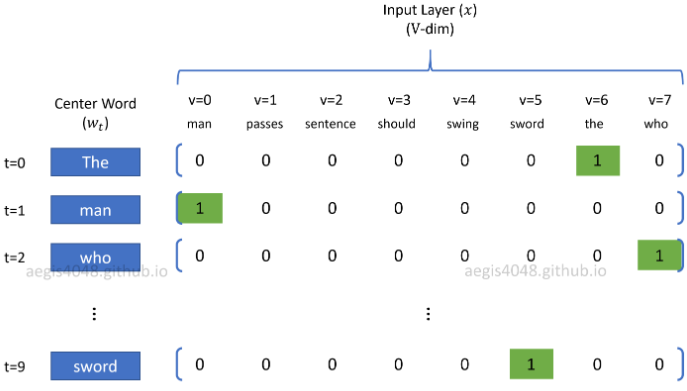
\includegraphics[width=0.7\linewidth]{pic/input_onehot.png}
            \caption{\scriptsize One-hot encoded input vector.}
        \end{figure} 
    \end{frame}

    \begin{frame}{Word2vec in action}   
        \begin{figure}[ht!]
            \centering
            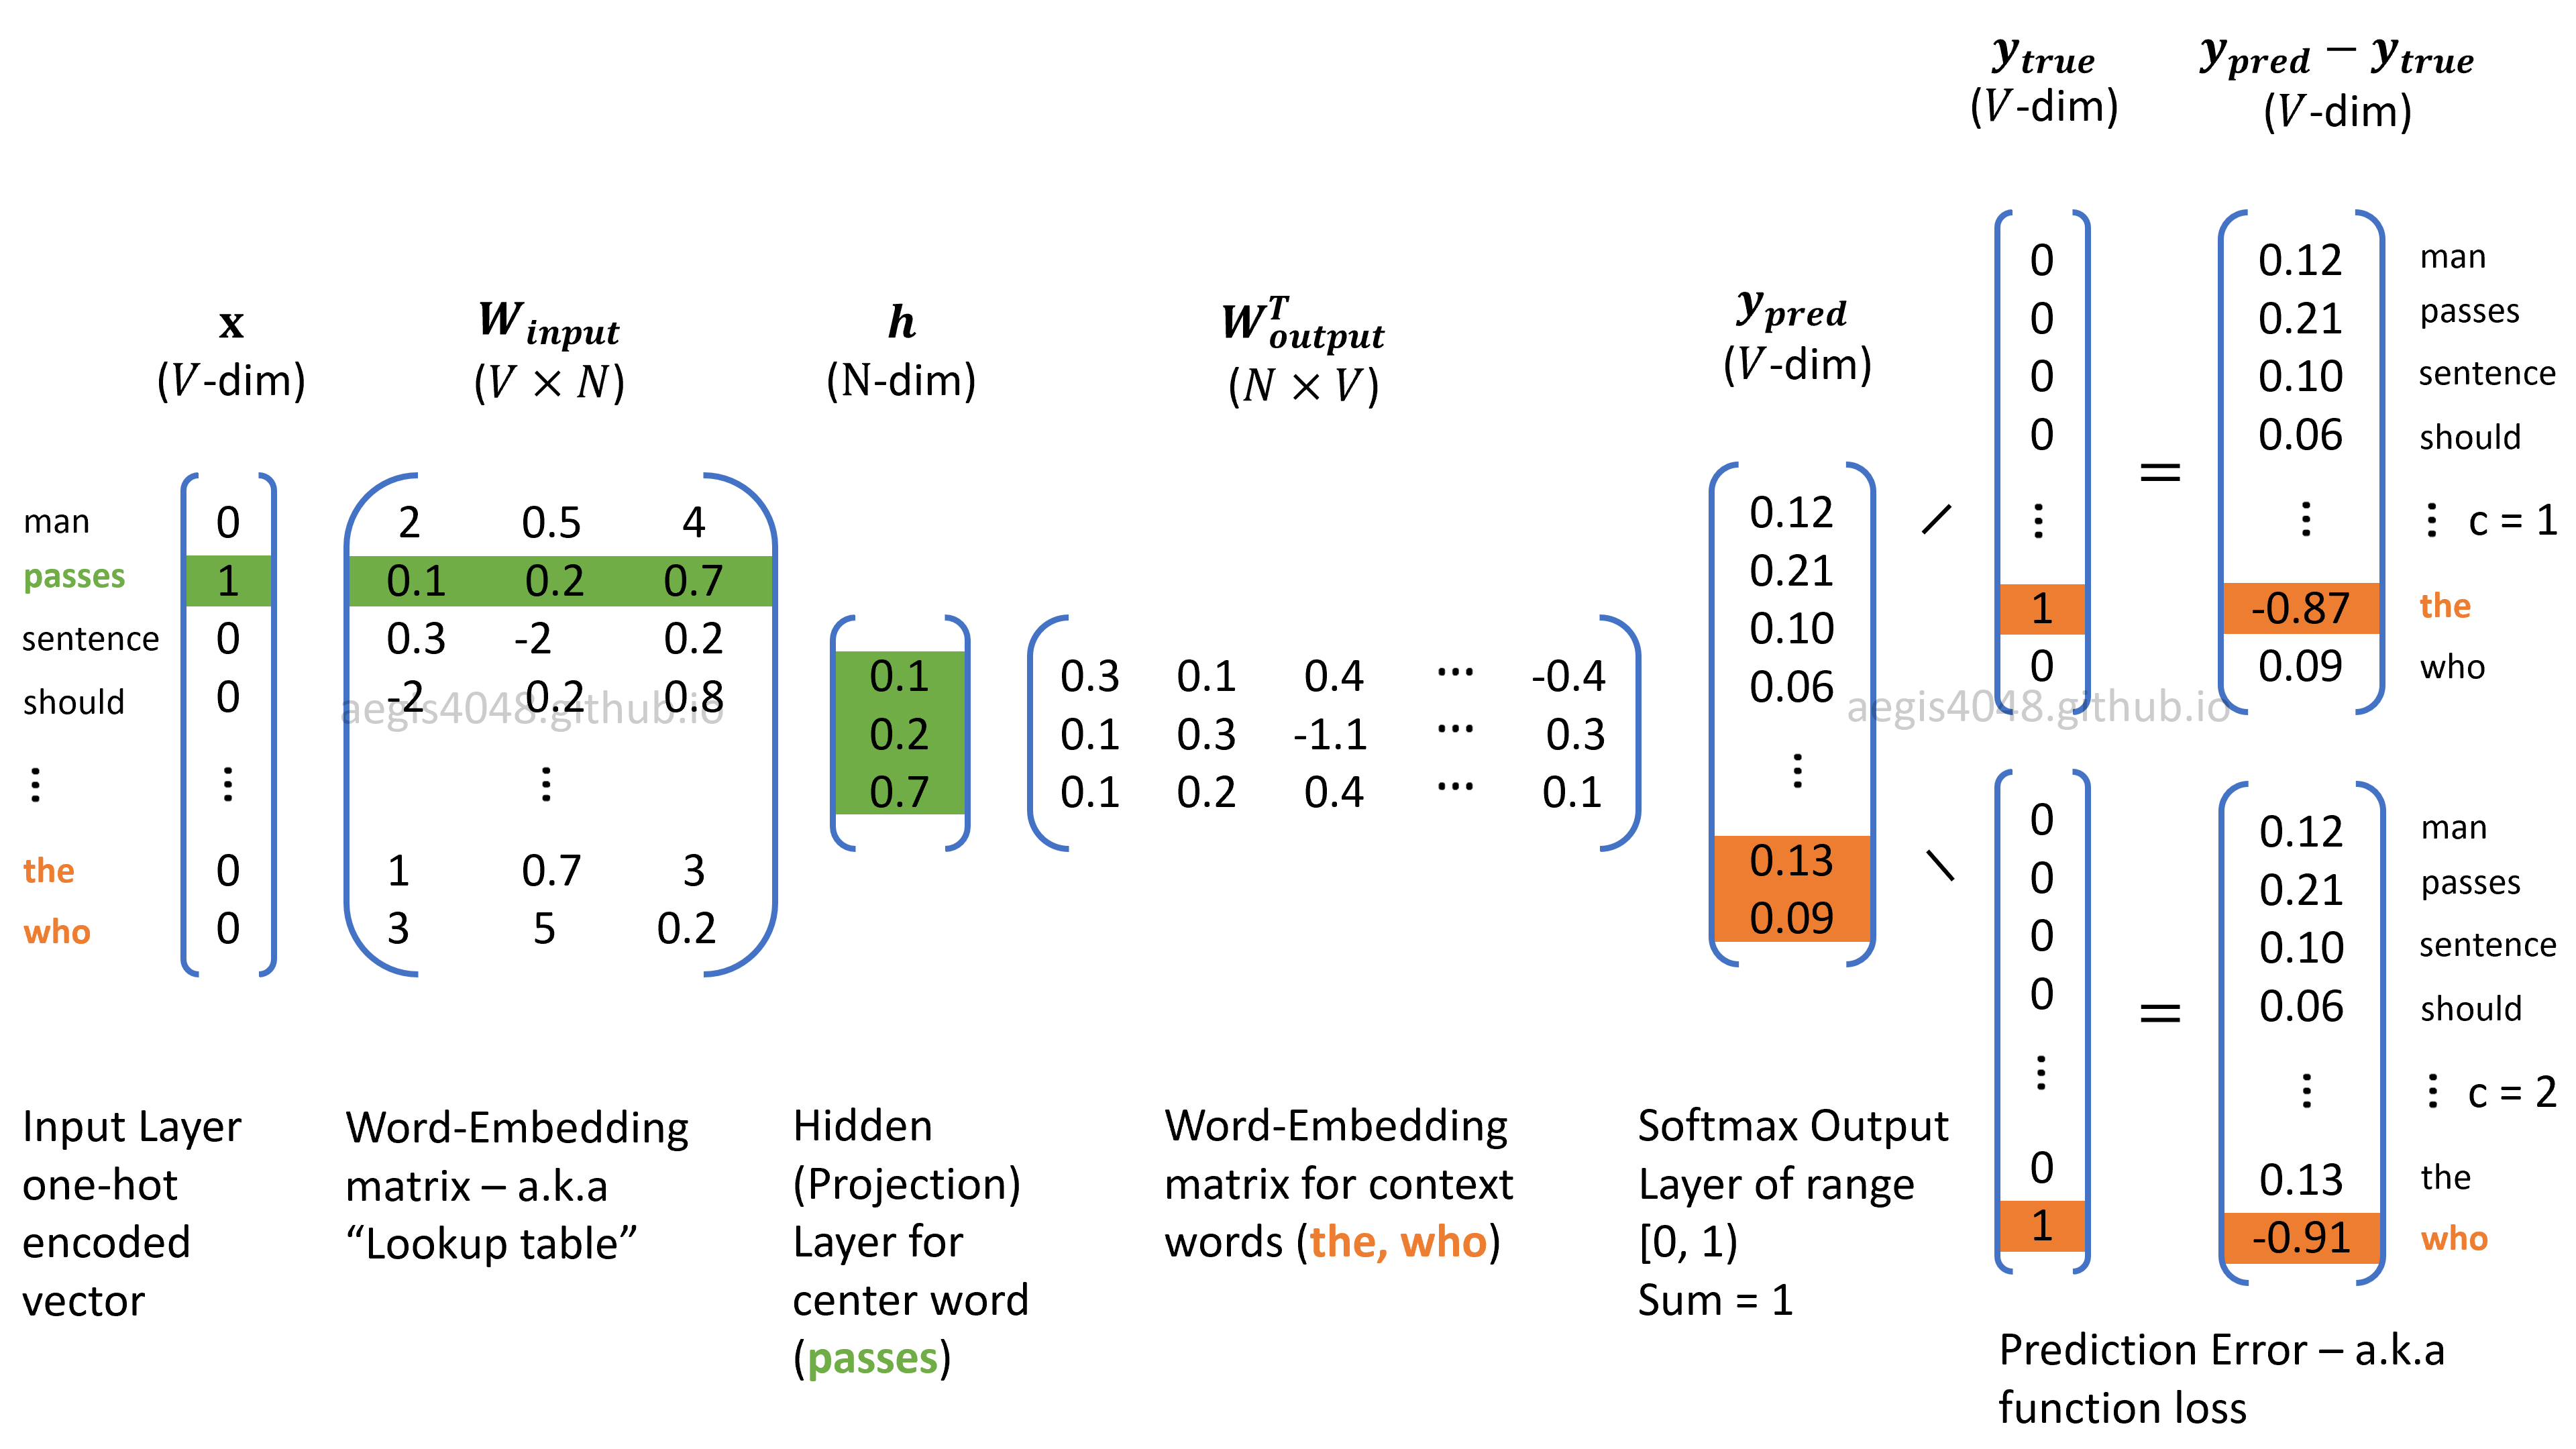
\includegraphics[width=1.0\linewidth]{pic/word2vec_skip-gram.png}
            \caption{\scriptsize Skip-Gram model structure. Current center word is ``passes''. From \url{https://aegis4048.github.io/demystifying_neural_network_in_skip_gram_language_modeling}.}
        \end{figure}   
    \end{frame}

    \begin{frame}{Word2vec in action}   
        \begin{figure}[ht!]
            \centering
            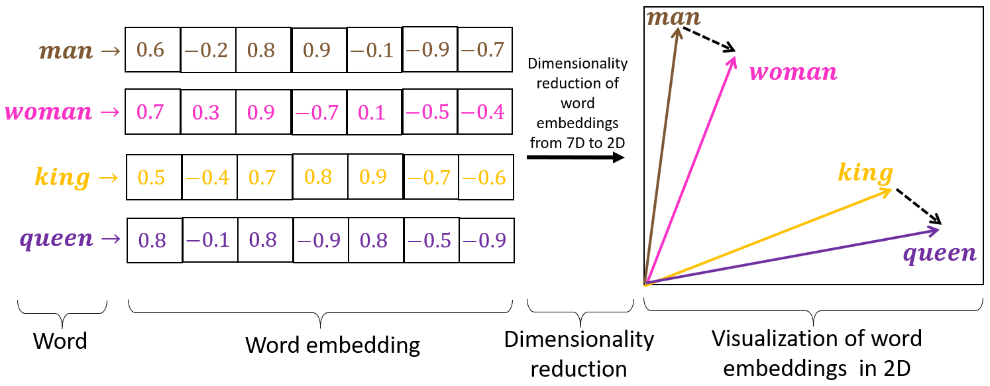
\includegraphics[width=0.85\linewidth]{pic/skip-gram_result.png}
            \caption{\scriptsize Word embeddings. \\
            From \url{https://doi.org/10.1371/journal.pone.0231189.g008}.}
        \end{figure}

        \centering
        Cosine similarity
        \begin{equation}
            cos(\theta) = \text{sim}(z_i, z_j) = \frac{z_i.z_j}{\|z_i\|\|z_j\|}
            \label{eq:cosine_similarity}
        \end{equation}
    \end{frame}

    \begin{frame}{DeepWalk \cite{mikolov2013distributed}}
        \begin{figure}[ht!]
            \centering
            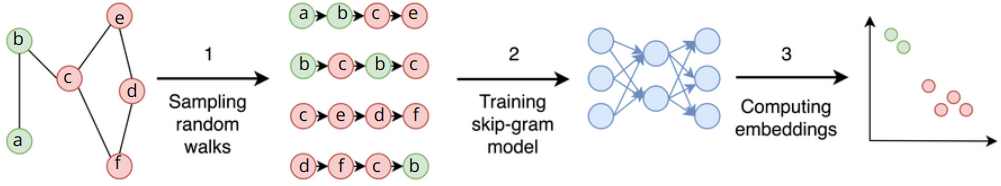
\includegraphics[width=1.0\linewidth]{pic/deepwalk.png}
            \caption{\scriptsize DeepWalk workflow.}
        \end{figure}

        Parameters:
        \begin{itemize}
            \item length = 4
            \item n = 1
        \end{itemize}
    \end{frame}

    \begin{frame}{Node2vec \cite{grover2016node2vec}} 
        \begin{figure}[ht!]
            \centering
            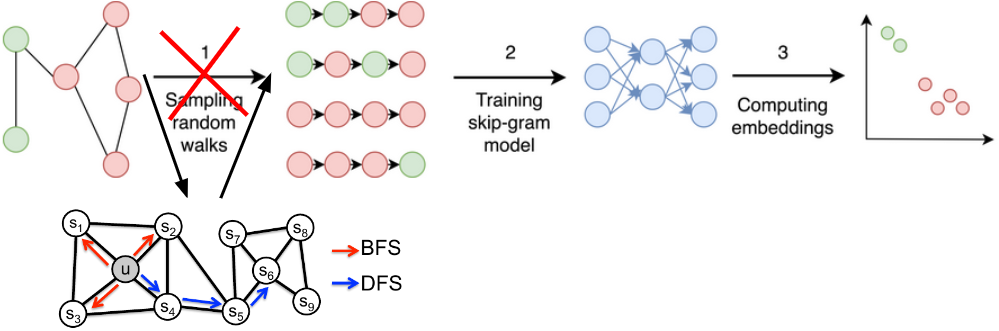
\includegraphics[width=1.0\linewidth]{pic/node2vec.png}
            \caption{\scriptsize Node2vec workflow.}
        \end{figure}

        Parameters:
        \begin{itemize}
            \item length = 4
            \item n = 1
            \item p = 1, q = 2 (BFS: micro-view) or
            \item p = 1, q = 0.5 (DFS: macro-view)
        \end{itemize}
    \end{frame}

    \begin{frame}{Application on biomedical data} 
        \begin{figure}[ht!]
            \centering
            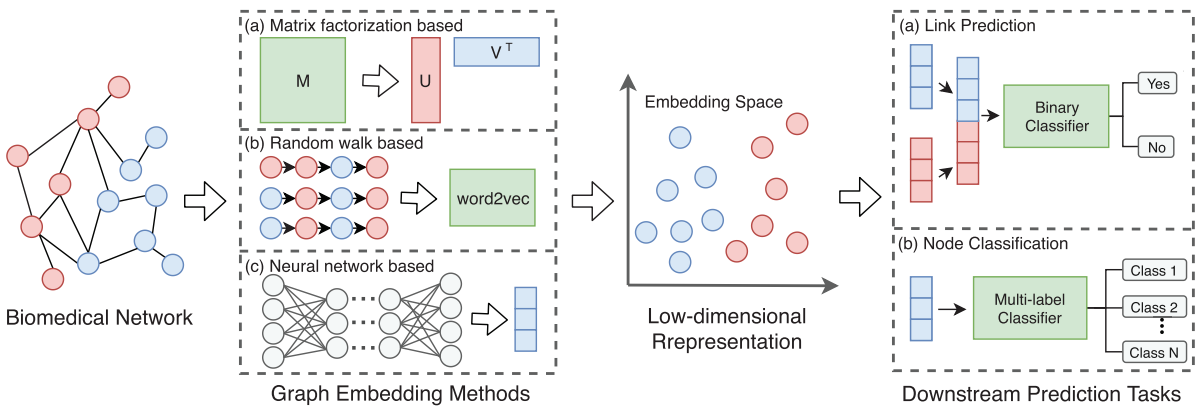
\includegraphics[width=1.0\linewidth]{pic/apply_graph_embedding.png}
            \caption{\scriptsize Applying graph embedding methods to biomedical tasks. Adapted from \cite{yue2020graph}.}
        \end{figure}
    \end{frame}

    \begin{frame}{Practical example: Node2vec} 
        \url{https://github.com/win7/Presentations-Hub/blob/main/SummerCamp-2025_IA-PUCP/Community_Detection.ipynb}
    \end{frame}

\section{Graph Neural Network (GNN)}
    
    \begin{frame}{Graph Neural Network (GNN)}
        \centering
        \LARGE GNN = Neural networks + Graph theory
    \end{frame}
    
    \begin{frame}{Basics of Neural networks (NN)}   
        \begin{figure}[ht!]
            \centering
            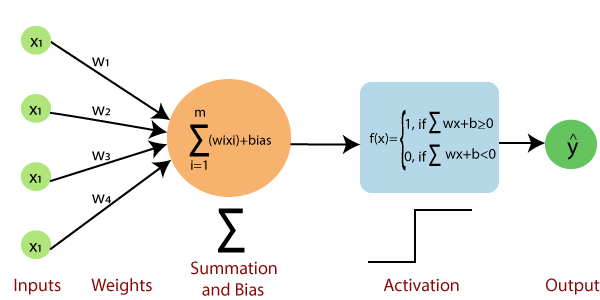
\includegraphics[width=0.86\linewidth]{pic/single-layer-perceptron-in-tensorflow2.png}
            \caption{\scriptsize Basic NN. \\
            From \url{https://www.javatpoint.com/single-layer-perceptron-in-tensorflow}.}
        \end{figure}   
    \end{frame}

    \begin{frame}{Neural networks (NN)}
        \begin{figure}[ht!]
            \centering
            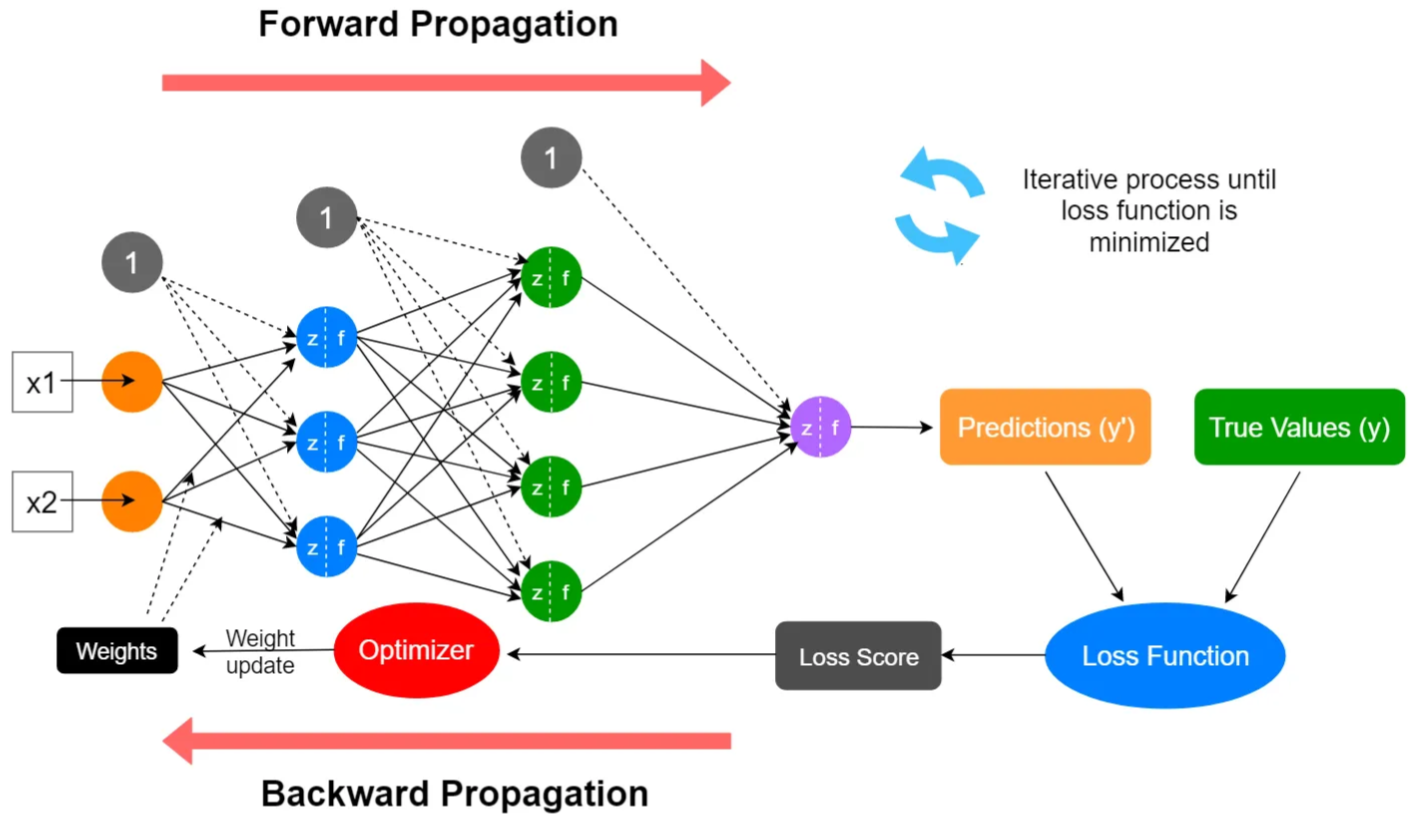
\includegraphics[width=1.0\linewidth]{pic/neural_networks.png}
            \caption{\scriptsize Basic NN. From \url{https://medium.com/data-science-365/overview-of-a-neural-networks-learning-process-61}.}
        \end{figure}   
    \end{frame}

    \begin{frame}{Example of NN}
        \begin{figure}
            \centering
            % \includegraphics{}
            \animategraphics[width=1.0\textwidth, loop, autoplay]
            {5} % frame rate
            {pic/network-propagation/network-propagation_} % path to figures
            {0} % start index
            {71} % end index
            \caption{Image classification. From \url{https://www.3blue1brown.com/lessons/neural-networks}.}
            \label{fig:example_nn}
        \end{figure}
    \end{frame}

    \begin{frame}{Graph Neural Networks (GNN)}
        It is a function $f: (A, X) \rightarrow H$ that maps each node of the graph $G = (V, E)$ into a $F$-dimensional vector. 
        \newline
        Here, $A \in \mathbb{R}^{N \times N}$,  $X \in \mathbb{R}^{N \times C}$, $H^{l} \in \mathbb{R}^{N \times F}$ with $F \ll N$, $l \in \{1, 2, ..., L\}$.
        
        % Usually, $z_i$ and $Z$ are called node embedding and embedding matrix, respectively.
        \centering
        $H = \text{GNN}(A, X)$
        \begin{figure}[ht!]
            \centering
            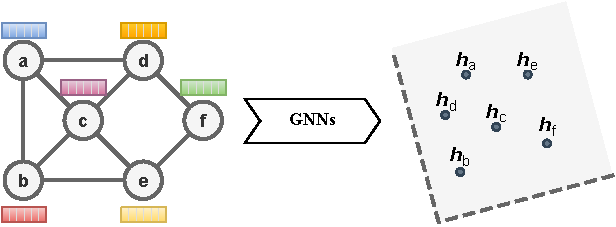
\includegraphics[width=0.7\linewidth]{pic/gnns.pdf}
            \caption{\scriptsize GNNs scheme.}
        \end{figure}               
    \end{frame}

    \begin{frame}{How GNNs works?}
        \begin{figure}[ht!]
            \centering
            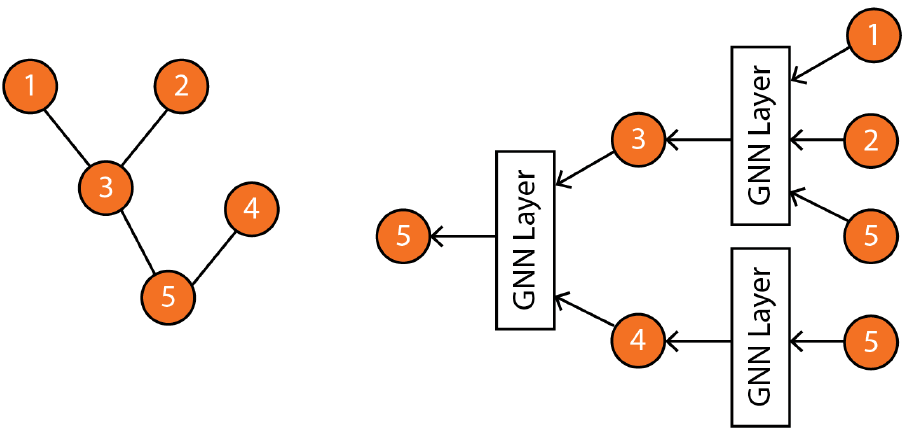
\includegraphics[width=0.7\linewidth]{pic/gnn_works.png}
            \caption{\scriptsize Computation graph representation. Adapted from \cite{labonne2023hands}.}
        \end{figure}               
    \end{frame}

    \begin{frame}{Tasks}
        \begin{figure}[ht!]
            \centering
            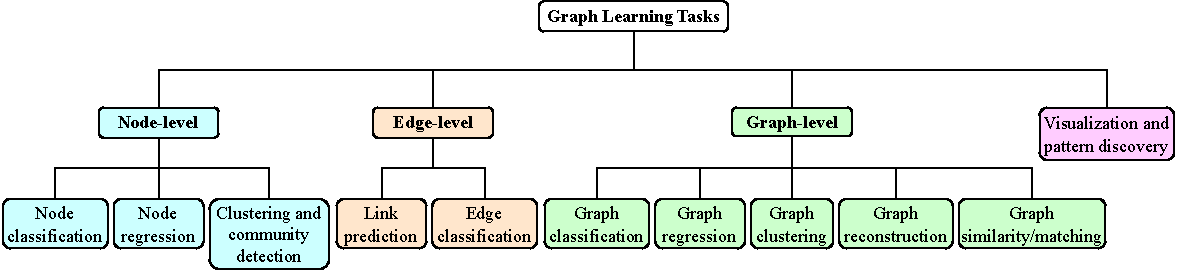
\includegraphics[width=1.0\linewidth]{pic/graph_learning_tasks.pdf}
            \caption{\scriptsize Overview of graph learning tasks.}
        \end{figure}               
    \end{frame}

    \begin{frame}{Taxonomy of graph machine learning methods.}
        \begin{figure}[ht!]
            \centering
            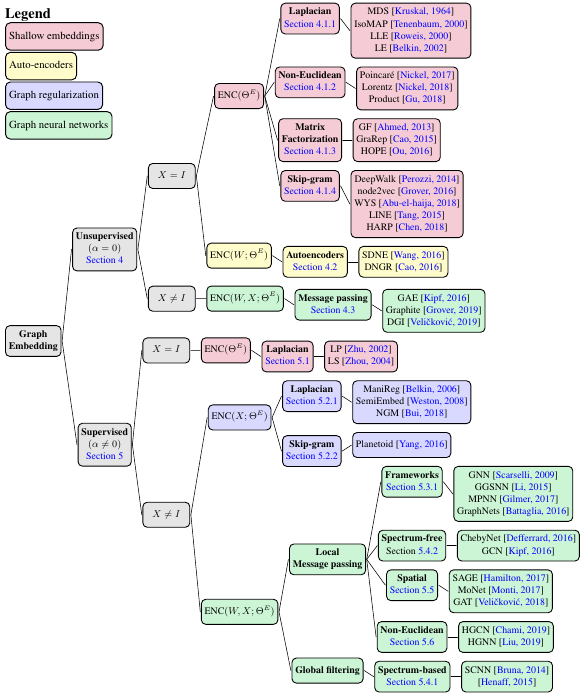
\includegraphics[width=0.512\linewidth]{pic/taxonomy_graph_machine_learning.png}
            \caption{\scriptsize Taxonomy of graph machine learning. Adapted from \cite{chami2022machine}.}
        \end{figure}               
    \end{frame}

    \begin{frame}{Variants of GNNs}
        \begin{itemize}
            \item Graph Convolutional Networks (GCN) \cite{kipf2016semi}
            % \item Graph Recurrent Networks (GRN)
            \item Graph Attention Networks (GAT) \cite{velickovic2017graph}
            \item Graph Isomorphism Networks (GIN) \cite{xu2018powerful}
            
            \item Variational Graph Auto-Eencoders (VGAE) \cite{kipf2016variational}
            \item Deep Graph Infomax (DGI) \cite{velivckovic2018deep}
            \item Adversarially Regularized Variational Graph Autoencoder (ARVGA) \cite{pan2018adversarially}
            \item Linear Graph Variational Autoencoder (LGVAE) \cite{salha2021simple}
            \item ...
        \end{itemize}
    \end{frame}

    \begin{frame}{Graph Convolutional Network (GCN)}
        \begin{figure}[ht!]
            \centering
            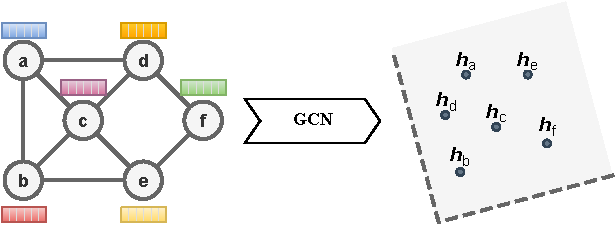
\includegraphics[width=0.7\linewidth]{pic/gcn.pdf}
            \caption{\scriptsize GCN scheme.}
        \end{figure}

        \begin{equation}
            H^{(l + 1)} = \sigma (\Tilde{D}^{-\frac{1}{2}} \Tilde{A} \Tilde{D}^{-\frac{1}{2}} H^{(l)} W^{(l)}) 
            \label{eq:propagation_gcn}
        \end{equation}

        Here, $\Tilde{A} = A + I_N$, $\Tilde{D}_{ii} = \sum_{j} \Tilde{A}_{ij}$, $W^{(l)}$ is trainable weight matrix, $\sigma(.)$ is an activation function.
    \end{frame}

    \begin{frame}{Application in computer vision}
        SuperGlue: Learning Feature Matching with Graph Neural Networks \cite{sarlin2020superglue}.
        
        \begin{figure}[ht!]
            \centering
            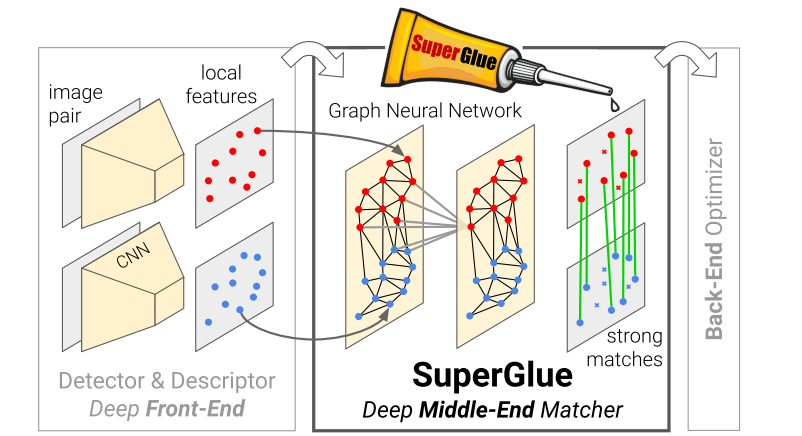
\includegraphics[width=0.7\linewidth]{pic/super_glue.png}
            \caption{\scriptsize SuperGlue scheme.}
        \end{figure}
    \end{frame}
    
    \begin{frame}{SuperGlue}
        \begin{figure}
            \centering
            % \includegraphics{}
            \animategraphics[width=\textwidth, loop, autoplay]
            {5} % frame rate
            {pic/imd/freiburg_matches-} % path to figures
            {0} % start index
            {15} % end index
            \caption{\scriptsize Matching example (indoor).}
            \label{fig:my_label}
        \end{figure}
    \end{frame}

    \begin{frame}{SuperGlue}
        \begin{figure}[ht!]
            \centering
            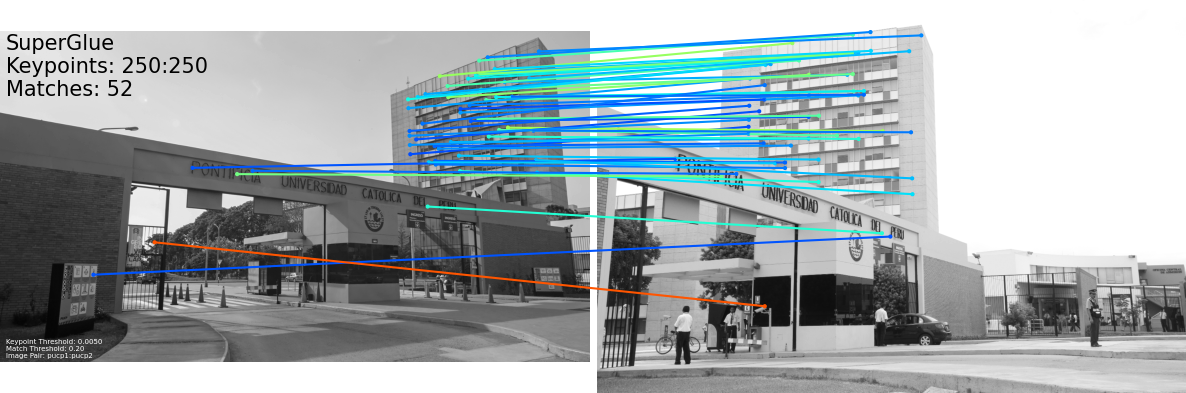
\includegraphics[width=1.0\linewidth]{pic/pucp1_pucp2_matches.png}
            \caption{\scriptsize Matching example (outdoor).}
        \end{figure}
    \end{frame}

    \begin{frame}{Application in recommender systems}
        Uber Eats
        \begin{figure}[ht!]
            \centering
            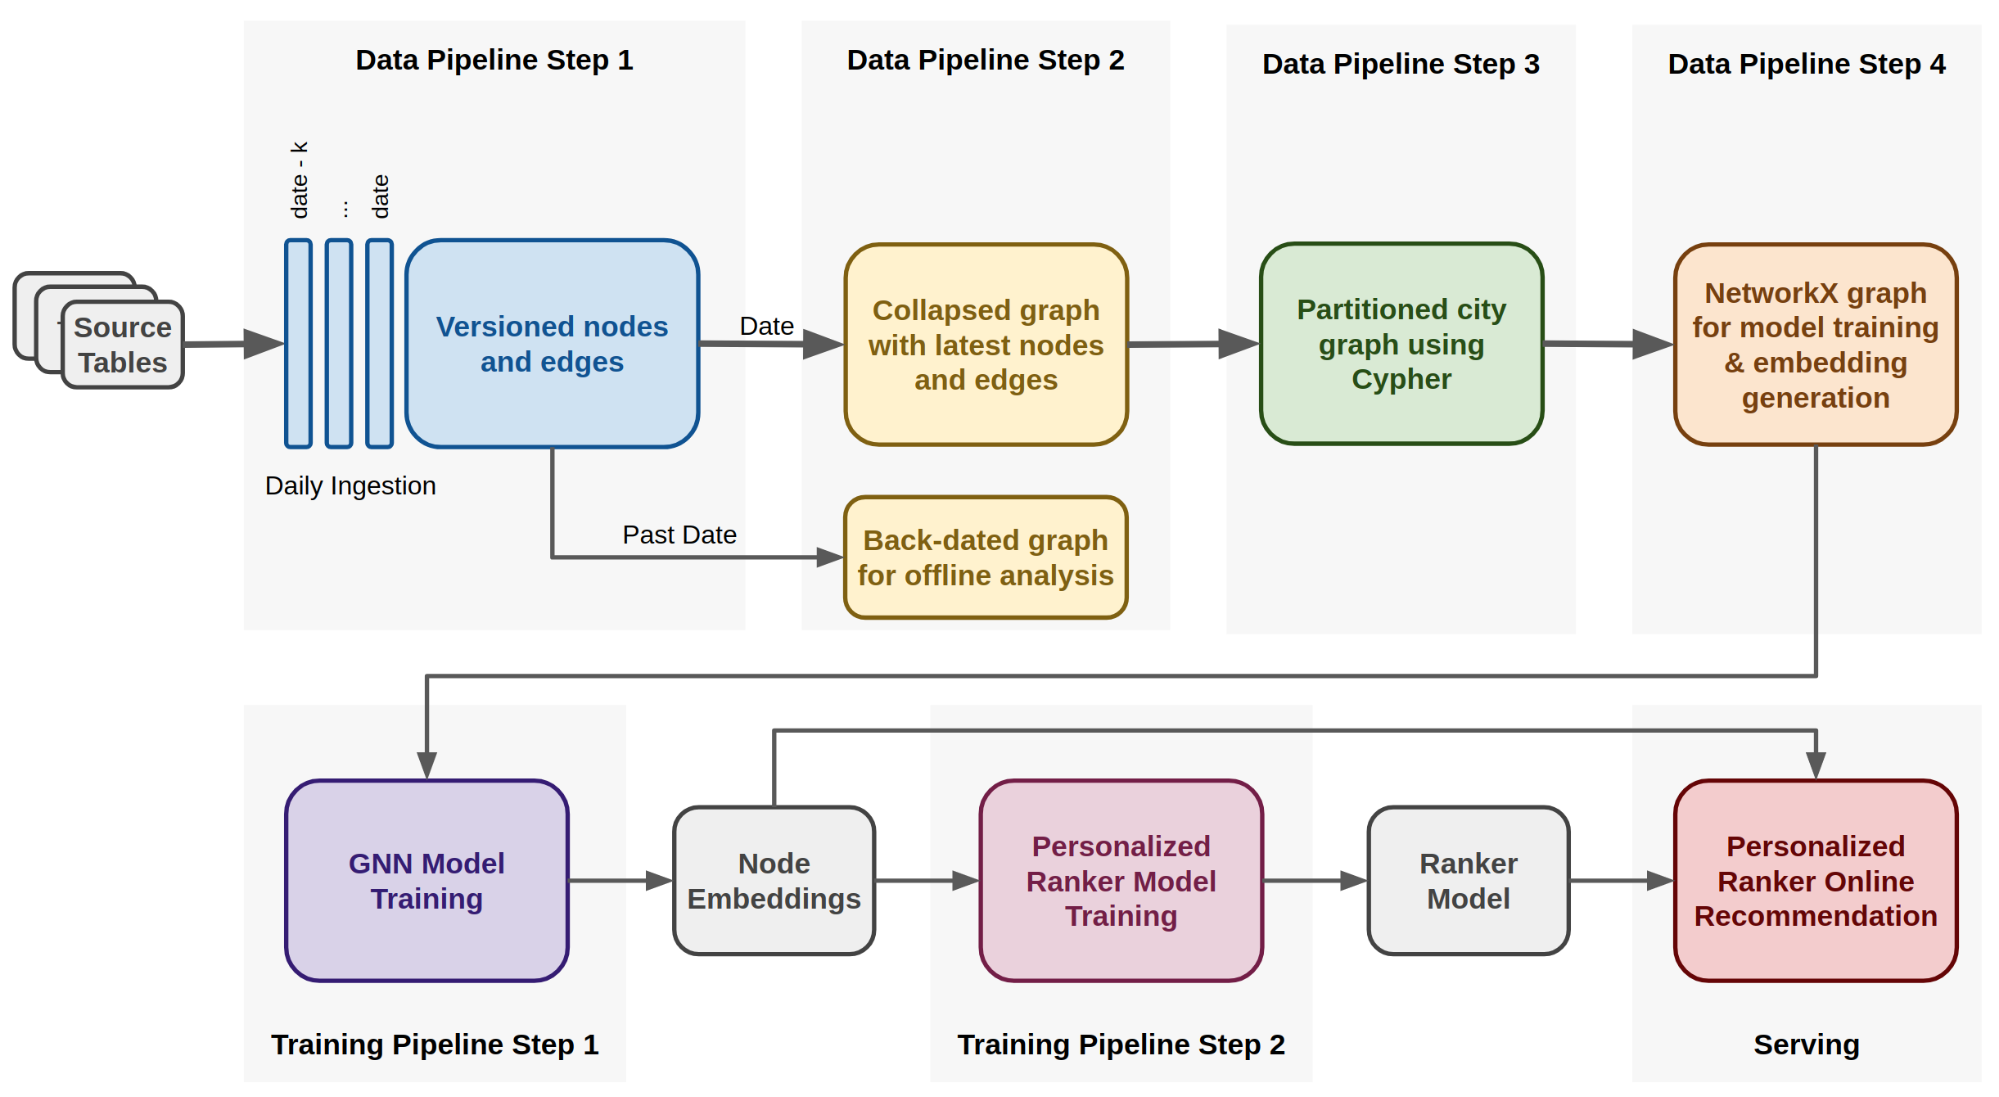
\includegraphics[width=0.9\linewidth]{pic/uber_model.png}
            \caption{\scriptsize Pipeline Uber eats. From \url{https://www.uber.com/en-CO/blog/uber-eats-graph-learning/}.}
        \end{figure}
    \end{frame}

    \begin{frame}{Uber Eats}
        \begin{figure}
            \centering
            % \includegraphics{}
            \animategraphics[width=0.35\textwidth, loop, autoplay]
            {5} % frame rate
            {pic/uber_eats/a733611516524151ebb9d28ad2c2ab68IaQ4dI3VB8Bs9CFt-} % path to figures
            {0} % start index
            {30} % end index
            \caption{\scriptsize Recommender systems example.}
            \label{fig:my_label}
        \end{figure}
    \end{frame}

    \begin{frame}{Practical example: GCN to node classification}
        \begin{figure}[ht!]
            \centering
            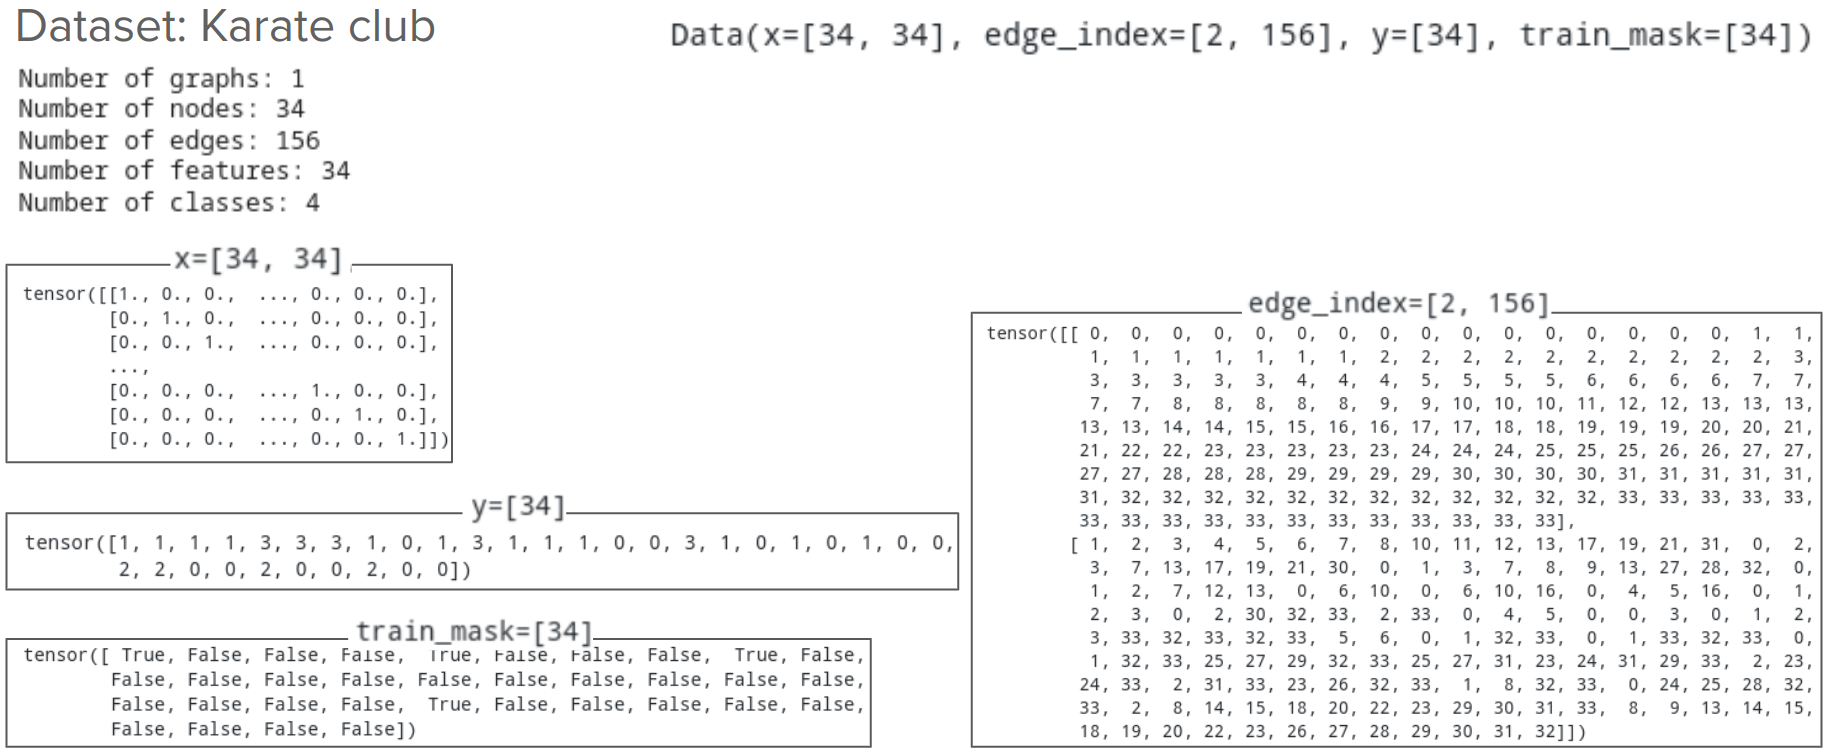
\includegraphics[width=1.0\linewidth]{pic/gcn_example.png}
            \caption{\scriptsize Karate club dataset.}
        \end{figure}
    \end{frame}

    \begin{frame}{Practical example: GCN to node classification}
        \begin{figure}
            \centering
            \begin{subfigure}{0.241\textwidth}
                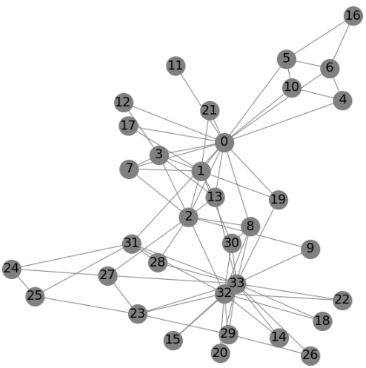
\includegraphics[width=1.0\textwidth]{pic/input_graph.png}
                \caption{\scriptsize Input graph.}
                \label{fig:first}
            \end{subfigure}
            \hfill
            \begin{subfigure}{0.241\textwidth}
                \centering
            % \includegraphics{}
            \animategraphics[width=1.3\textwidth, loop, autoplay]
            {5} % frame rate
            {pic/train_gcn/download_} % path to figures
            {0} % start index
            {149} % end index
            \caption{Train GCN.}
            \label{fig:my_label}
            \end{subfigure}
            \hfill
            \begin{subfigure}{0.241\textwidth}
                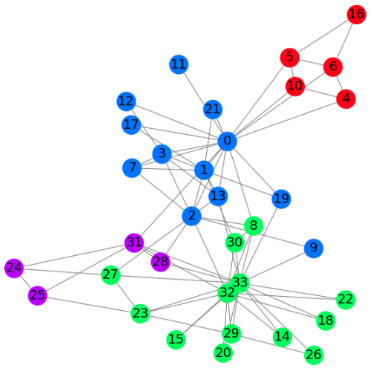
\includegraphics[width=\textwidth]{pic/output_graph.png}
                \caption{\scriptsize Output graph.}
                \label{fig:third}
            \end{subfigure}
            \caption{\scriptsize GCN to node classification.}
            \label{fig:graph_representation}
        \end{figure}                     
    \end{frame}

    \begin{frame}{Practical example: GCN to node classification} 
        \url{https://github.com/win7/Presentations-Hub/blob/main/SummerCamp-2025_IA-PUCP/Node_Classification.ipynb}
    \end{frame}

\section{Resources}
    \begin{frame}{Package, library, and framework}        
        \begin{figure}[ht!]
            \centering
            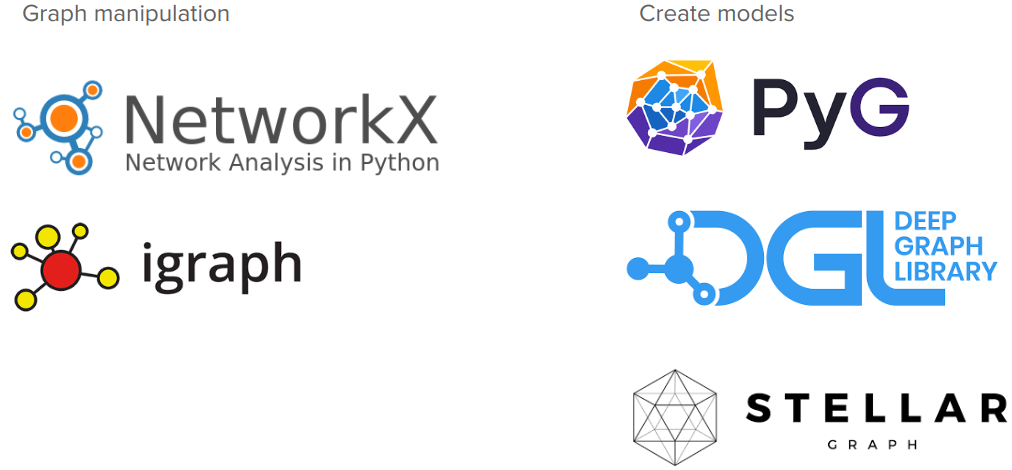
\includegraphics[width=0.9\linewidth]{pic/sources.png}
            \caption{\scriptsize Package, library, and framework.}
        \end{figure}               
    \end{frame}

    \begin{frame}{Books}        
        \begin{figure}[ht!]
            \centering
            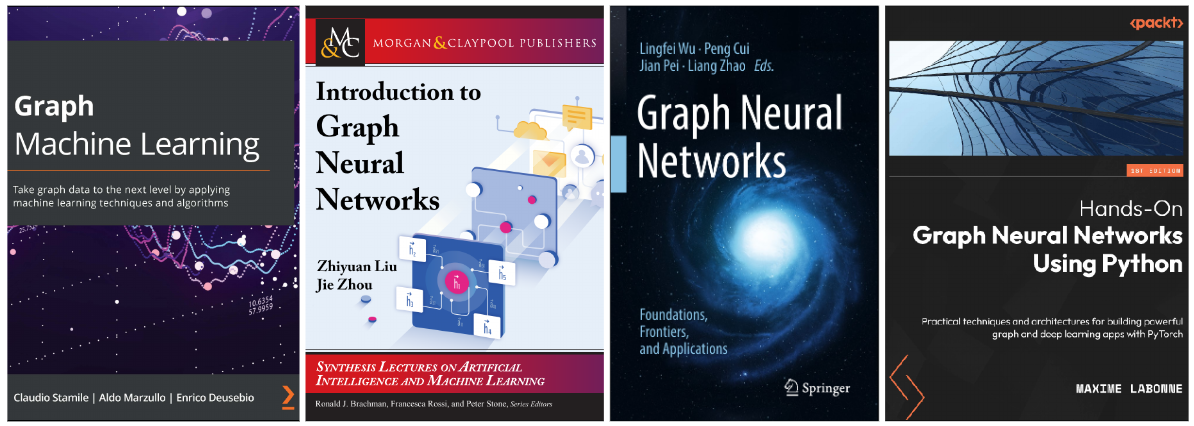
\includegraphics[width=1.0\linewidth]{pic/books_source.png}
            \caption{\scriptsize GNNs books.}
        \end{figure}               
    \end{frame}

    \begin{frame}{More learning}
        \begin{itemize}
            \item Courses
            \begin{itemize}
                \item CS224W: Machine Learning with Graphs \\ (\url{http://web.stanford.edu/class/cs224w/})
            \end{itemize}
            \item Tutorials
            \begin{itemize}
                \item PyTorch Geometric: Introduction by Example \\ (\url{https://pytorch-geometric.readthedocs.io/en/latest/notes/introduction.html})
            \end{itemize}
            \item Conferences
            \begin{itemize}
                \item Learning on Graphs \\ (\url{https://logconference.org/})
            \end{itemize}
        \end{itemize}
    \end{frame}

\begin{frame}[allowframebreaks]
    % \bibliography{ref}
    % \bibliographystyle{unsrt}
    % \bibliographystyle{alpha}
    % If too many references, use this command to resize：
    % \tiny\bibliographystyle{unsrt}
\end{frame}

\begin{frame}
    \begin{center}
        {\Huge\textit{Thank you for your attention!}}\\
        $\infty$ \\
        edwin.alvarez@pucp.edu.pe\\
        \url{https://github.com/win7}
    \end{center}
\end{frame}

%========================
% bibliographya
%========================
% \input{ref.bib}

\end{document}